\chapter{Metodologia}

Neste capítulo será detalhado os três módulos propostos na figura \ref{fig:proposta}: 
Condições Iniciais, Treinamento e Geração de Sequências. 
Além disso, será apresentado os métodos de avaliação das proteínas geradas,
bem como as especificações de hardware e software utilizados. 


\section{Condições iniciais}
O objetivo do primeiro módulo (figura \ref{fig:cond_iniciais}) é obter a sequência ($S_{ini}$) e o erro ($Er_{0}$) iniciais. 
A primeira é obtida ao se passar a estrutura alvo como entrada do \textit{ProteinMPNN}.
Já o erro inicial é definido pela seguinte expressão:
 
\begin{equation}
    Er_{0} = 1 - TMScore(E_{FIX}, E_{ini})
\end{equation}

\noindent
Onde $E_{FIX}$ é a estrutura alvo, i.e, a estrutura do fator IX de coagulação e $E_{ini}$ é a estrutura vinculada a sequência inicial, 
predita pelo \textit{ESMFold} - descrito em \ref{subsection:structure_pred}. 
O \textit{TMScore} consiste em uma medida de similariedade entre estruturas, detalhada em \ref{subsection:TMScore}

\begin{figure}[H]
  \centering
  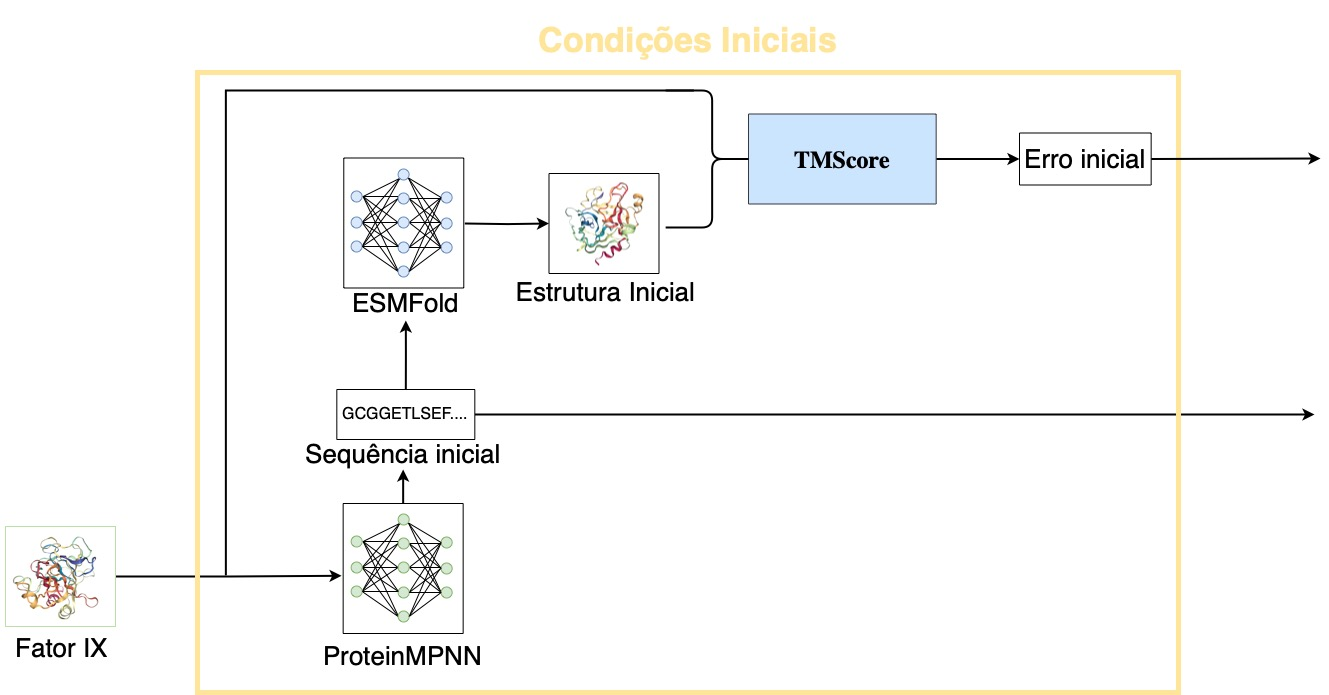
\includegraphics[width=.8\textwidth]{figuras/metodologia-Initial_cond.jpg}
  \caption{Obtenção das condições iniciais}
  \label{fig:cond_iniciais}
\end{figure}

\begin{algorithm}
  \caption{Obtenção das Condições Iniciais}
  \label{alg:initial_conditions}
  \begin{algorithmic}[1]
  \Require Estrutura alvo $E_{FIX}$
  \Ensure Sequência inicial $S_{ini}$ e erro inicial $Er_{0}$
  \State $S_{ini} \gets \textit{ProteinMPNN}(E_{FIX})$
  \State $E_{ini} \gets \textit{ESMFold}(S_{ini})$
  \State $Er_{0} \gets 1 - \textit{TMScore}(E_{FIX}, E_{ini})$
  \State \Return $S_{ini}, Er_{0}$
  \end{algorithmic}
  \end{algorithm}

Esta implementação\footnote{Disponível em: \url{https://github.com/ArthurPimenta0306/Hallucination/blob/main/hpd/src/hpd/pipelines/Modeling/nodes.py}},
bem como seu comando para execução\footnote{\texttt{kedro run mo\_get\_initial\_conditions --nodes get\_initial\_conditions\_B\_node}} estão  
disponíveis.
As parametrizações e os comandos para execução utilizadas no \textit{ProteinMPNN}, \textit{ESMFold} e \textit{TMScore} são apresentadas a seguir:

\textbf{Comando para execução - \textit{ProteinMPNN}}
\begin{lstlisting}[language=bash, breaklines=true, frame=single, backgroundcolor=\color{lightgray}]
  python src/ProteinMPNN/protein_mpnn_run.py \
      --pdb_path {structure_path} \
      --pdb_path_chains {chains_to_design} \
      --out_folder tmp \
      --num_seq_per_target 1 \
      --sampling_temp "0.5" \
      --seed 37 \
      --batch_size 1
  \end{lstlisting}
\textbf{Parametrização - \textit{ProteinMPNN}}
\begin{enumerate}
    \item \textbf{pdb\_path}: \texttt{data/05\_model\_input/fixa\_human\_SP\_renumber.pdb}. Caminho até o arquivo da estrutura do FIX. 
    \item \textbf{pdb\_path\_chains}: \texttt{"H"}. Cadeia proteica a ser predita. 
    \item \textbf{out\_folder}: \texttt{"tmp"}. Nome do diretório temporário. 
    \item \textbf{num\_seq\_per\_target}: \texttt{1}. Quantidade de sequências geradas. 
    \item \textbf{sampling\_temp}: \texttt{0.5}. Temperatura de amostragem. Quanto menor, mais conservadora a predição. 
    \item \textbf{seed}: \texttt{37}. Semente aleatória para reprodutibilidade da predição.
    \item \textbf{batch\_size}: \texttt{1}. Tamanho do batch utilizado para inferência. 
\end{enumerate}

\textbf{Comando para execução - \textit{ESMFold}}
\begin{lstlisting}[language=bash, breaklines=true, frame=single, backgroundcolor=\color{lightgray}]
  curl -X POST --data "{initial_seq}" https://api.esmatlas.com/foldSequence/v1/pdb/ > tmp/pred_initial_structure.pdb
\end{lstlisting}

\textbf{Parametrização - \textit{ESMFold}}
\begin{enumerate}
    \item \textbf{data}: String contendo a sequência de aminoácidos. Ex: "AACYA...".
\end{enumerate}


\textbf{Comando para execução - \textit{TMScore}}
\begin{lstlisting}[language=bash, breaklines=true, frame=single, backgroundcolor=\color{lightgray}]
  ./USalign -outfmt 2 {path_structure_1} {path_structure_2}
\end{lstlisting}

\textbf{Parametrização - \textit{TMScore}}
\begin{enumerate}
    \item \textbf{path\_structure\_1}: Caminho até o arquivo .pdb da estrutura protéica referência. 
    \item \textbf{path\_structure\_2}: Caminho até o arquivo .pdb da segunda estrutura protéica a ser comparada. 
\end{enumerate}

\section{Treinamento}
O módulo de Treinamento foi construído em duas etapas: Estágios I e II, detalhados em \ref{subsection:stage1} e \ref{subsection:stage2} respectivamente.
Para ambos os estágios, o treinamento se dá através de interações entre dois componentes: O Ambiente de aprendizado e o Agente. 

\subsection{Ambiente de aprendizado}
O ambiente de aprendizado é modelado como um MDP e, portanto, é responsável por definir o espaço de ações, o espaço de estados, a função de transição entre estados dado uma ação e a função de recompensa.  

\subsubsection{Espaço de ações}

Definimos uma ação como um vetor bi-dimensional composto pelo índice $p$ de uma posição na sequência e um aminoácido $r$. 
A ação será utilizada para realizar uma mutação na proteína, inserindo o $r$ na posição $p$. 
De modo a incentivar o Agente a explorar diferentes ações, 
definimos, para cada iteração, um conjunto de posições e aminoácidos válidos: $P_{val}$ e $R_{val}$ respectivamente. 
$P_{val}$ é composto por todas as possíveis posições na sequência, com exceção das posições previamente selecionadas dentro do mesmo episódio. 
Definimos $R_{val}$ sendo igual aos 20 possíveis aminoácidos, com exceção dos aminoácidos que foram selecionados 
mais do que $N_{rep}$ vezes. Introduzimos $N_{rep}$ como um hiperparâmetro que define a quantidade máxima 
permitida que um mesmo resíduo pode ser selecionado dentro de um episódio.   %7 vezes no mesmo episódio. 
Desta forma, o espaço de ações, para cada iteração $i$, é definido por:

\begin{equation}
A_{i} = \left\{(p, r) | p \in P_{val_{i}} , r \in R_{val_{i}} \right\}
\end{equation}
  

\subsubsection{Espaço de estados}
Definimos o espaço de estados como o conjunto de todas as possíveis sequências de $n$ aminoácidos, 
onde $n$ é o tamanho da sequência inicial:

\begin{equation}
S = \left\{(r_{1}, r_{2}, r_{3}, ..., r_{n}) | r_{i} \in R_{encoded} \forall i \in [1,n] \right\}
\end{equation}

Onde $R_{encoded}$ é o conjunto dos 20 possíveis aminoácidos, 
cada um representado por um vetor codificado pelo \textit{Encoder}. 
O \textit{Encoder} consiste em um dicionário que mapeia cada aminoácido para 
uma representação vetorial que conserva as distâncias entre cada par de aminoácidos estabelecidas por \cite{aminodist}.
Este mapeamento foi construído através de um MDS\footnote{Implementação do MDS construída pelo pacote scikit learn, disponível em: \url{https://scikit-learn.org/stable/modules/generated/sklearn.manifold.MDS.html}} utilizando 21 dimensões. 

\begin{figure}[H]
  \centering
  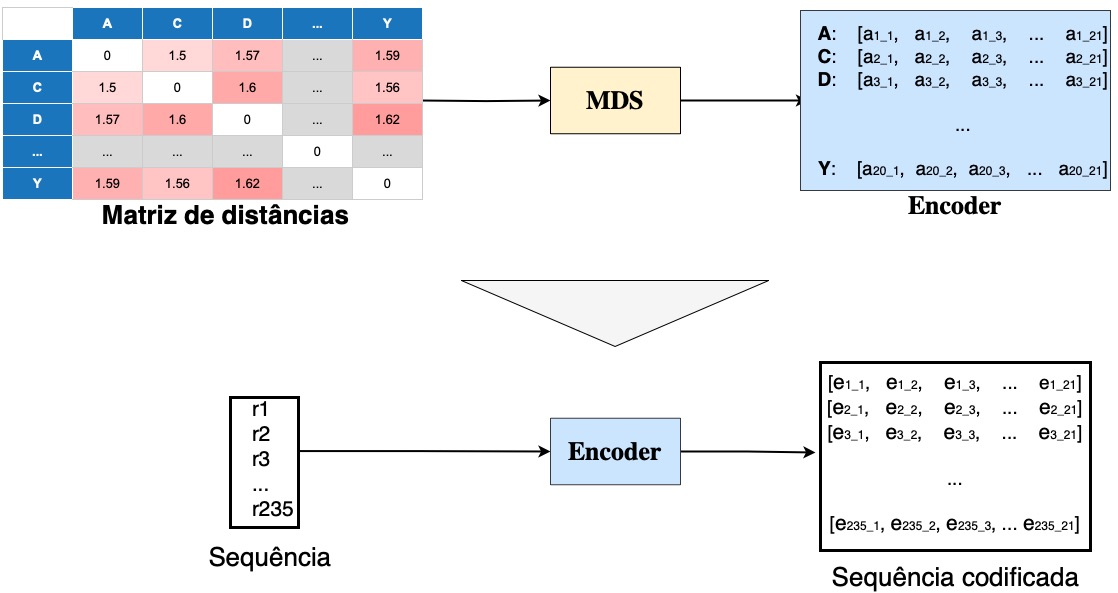
\includegraphics[width=.8\textwidth]{figuras/metodologia-encoder.jpg}
  \caption{Construção e uso do \textit{Encoder}. }
  \label{fig:encoder}
\end{figure}

Para escolher a quantidade de dimensões a se utilizar no MDS, 
definimos o ponto a partir do qual a curva\footnote{Disponível na seção "Encoding Aminoácidos" em \url{https://github.com/ArthurPimenta0306/Hallucination/blob/main/hpd/notebooks/GeneralAnalysis.ipynb}} entre \textit{Stress} e dimensionalidade 
tende a se aproximar assintóticamente do eixo x do plano cartesiano. 
Este ponto, conforme a figura \ref{fig:best_dim}, é o que possui 21 dimensões. 

\begin{figure}[H]
  \centering
  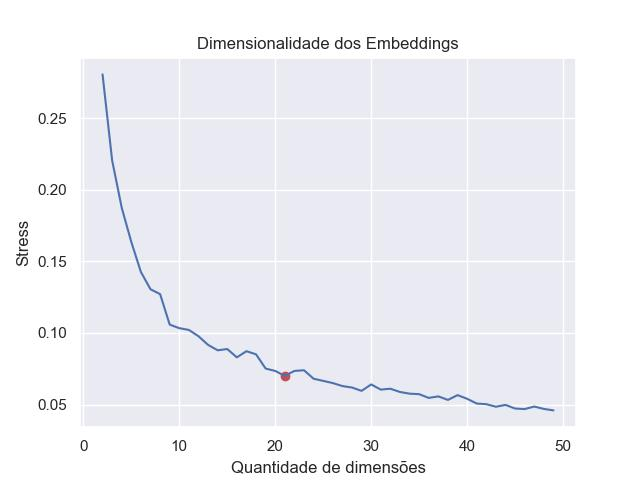
\includegraphics[width=.8\textwidth]{figuras/best_dim.jpg}
  \caption{Escolha da dimensionalidade dos Embeddings}
  \label{fig:best_dim}
\end{figure}


\subsubsection{Função de transição de estados}
A função de transição de estados é caracterizada pela geração de uma nova sequência, 
resultante da mutação definida pelo Agente. 
Em outras palavras, é uma função que tem como entrada uma ação e o estado atual e como saída o estado resultante da transição. 

\begin{figure}[H]
  \centering
  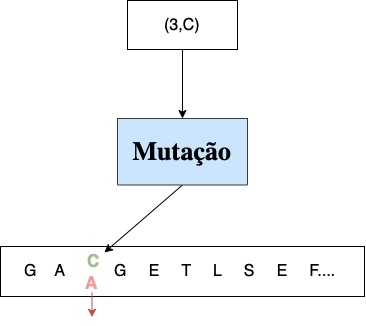
\includegraphics[width=.5\textwidth]{figuras/metodologia-Mutation.jpg}
  \caption{Exemplo de mutação. O aminoácido A na posição 3 está sendo substituído pelo o aminoácido C}
  \label{fig:mutacao}
\end{figure}

\subsubsection{Função de recompensa}
Já a função de recompensa calcula a qualidade da ação selecionada pelo Agente. 
Nas seções \ref{subsection:stage1} e \ref{subsection:stage2} especificamos a função de recompensa de cada estágio de treinamento.


\subsection{Agente}
\label{subsection:Agente}
O Agente é modelado por uma rede neural, batizada de \textit{GenSeq}, 
cujos parâmetros são otimizados através da técnica 
\textit{Proximal Policy Optimization} (PPO)\footnote{Implementação do PPO construída pelo pacote stable baselines, disponível em: \url{https://github.com/Stable-Baselines-Team/stable-baselines3-contrib/tree/master/sb3_contrib/ppo_mask}}, 
sendo responsável por decidir qual a melhor mutação a se fazer, dada a sequência de entrada. Em outras palavras, o Agente deve escolher,
dentro do espaço de ações, a ação que maximiza a recompensa acumulada.
Os hiperparâmetros utilizados no Agente são apresentados na tabela a seguir. 

\begin{table}[H]
\centering
\vspace{0.5cm}
\begin{tabular}{r|lr}
Hiperparâmetro & Valor \\ 
\hline                               
Número de camadas escodidas & 2 \\
Número de neurônios por camada escondida & 64 \\
Função de ativação & tangente hiperbólica \\
Otimizador & Adam \\
Taxa de aprendizagem & 3e-4 \\
Número de épocas & 10 \\
Fator de desconto ($\gamma$) & 0.99 \\
\end{tabular}
\caption{Hiperparâmetros do PPO}
\end{table}

Após ser processada pelo \textit{Encoder}, a sequência passa pela camada de entrada do \textit{GenSeq} e 
segue para duas camadas escondidas de 64 dimensões cada. 
A camada de saída, por sua vez, possui 255 unidades, organizadas em duas partes:

\begin{enumerate}
  \item As primeiras 235 unidades da camadas estão associadas ao primeiro atributo da ação: A posição $p$ da sequência de entrada
  que deve sofrer mutação. A posição predita pelo Agente corresponde ao índice da unidade de saída com maior valor entre as 235 primeiras. 
  \item Já as 20 últimas unidades de saída estão associadas ao segundo atributo da ação: O índice do aminoácido $r$ que o Agente sugere inserir na posição $p$.
  Este valor corresponde ao índice da unidade de saída com maior valor entre as 20 últimas unidades, subtraído de 235.
\end{enumerate}

Por exemplo, suponha que, entre as 235 primeiras unidades, a de maior valor é a terceira, e que, entre as 20 útltimas, o maior valor esteja na unidade 240. 
Nesse caso, a ação sugerida pelo Agente é fazer uma mutação na posição 3, inserindo o aminoácido de índice 5.

\begin{figure}[H]
  \centering
  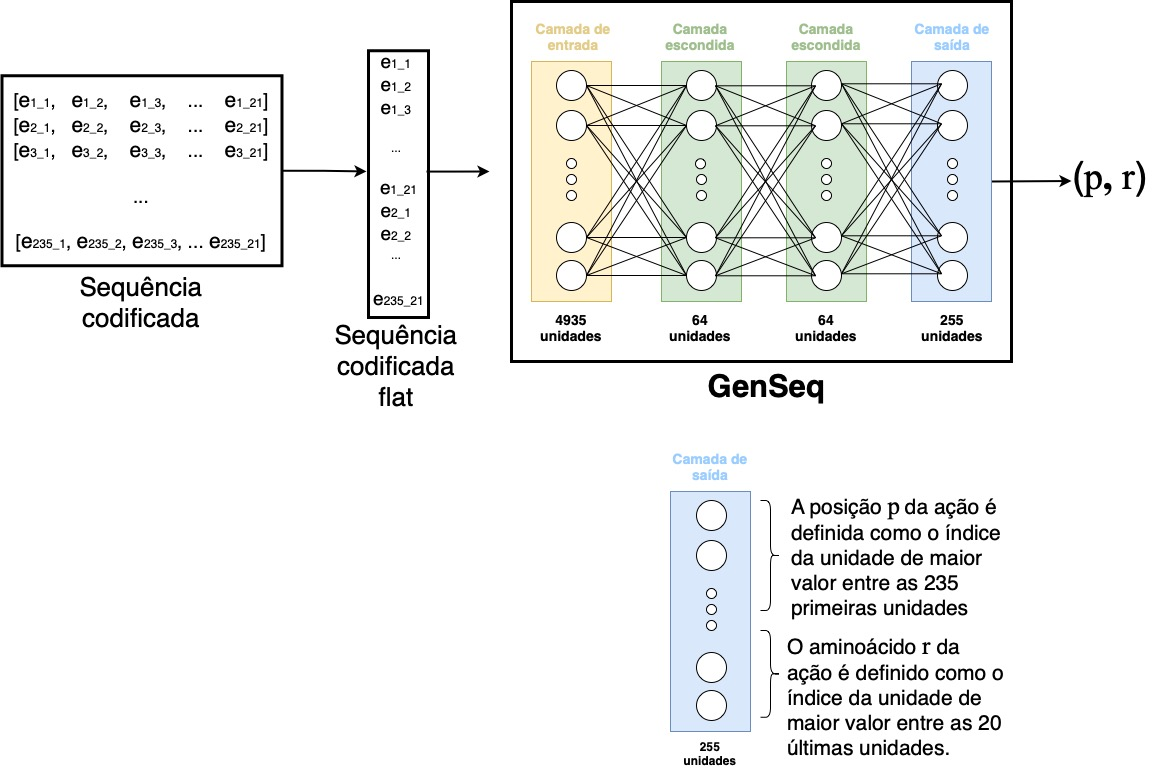
\includegraphics[width=.8\textwidth]{figuras/metodologia-NN_arch_actor.jpg}
  \caption{Arquitetura da rede neural do Agente (\textit{GenSeq})}
  \label{fig:actor_arch}
\end{figure}


\subsection{Treinamento - Estágio I}
\label{subsection:stage1}
%Definição de episodio 
%Vitoria ou derrota no episodio
%Numero de steps total e por episodio

Tendo em vista o vasto número de ações possíveis, 
desenvolvemos o Estágio I de treinamento com o objetivo de estimular o Agente a encontrar um subespaço menor de ações para atuar.
Neste estágio, construímos o ambiente de aprendizado $EnvI$, onde atribuímos recompensas negativas (ou penalizações) 
para ações em posições da sequência cujo o \textit{Conservation Score} \ref{subsection:CS} é alto,
bem como penalizamos ações onde o aminoácido substituído é muito diferente do que fora inserido. 
Neste sentido, definimos a seguinte função de recompensa:

\begin{equation}
    R_{I} = -(CS(p) + AminoDist(r, r_{prev}))
\end{equation}

\noindent
Onde $p$ e $r$ são a posição e o aminoácido selecionados pelo Agente, respectivamente. 
O $r_{prev}$ é o aminoácido que estava na posição $p$ antes da mutação. 
$CS(p)$ é o \textit{Conservation Score} normalizado da posição $p$ e $AminoDist(r, r_{prev})$ 
é a medida de similariedade \ref{subsection:AminoDist} entre os aminoácidos $r$ e $r_{prev}$.

O ambiente $EnvI$ foi construído seguindo a padronização proposta 
pelo pacote \textit{gym}\footnote{GYM, API padrão para ambientes de aprendizado por reforço, disponível em: \url{https://www.gymlibrary.dev/}} 
que garante compatibilidade com algoritmos de aprendizado por reforço.
Como entrada, o ambiente recebe uma sequência inicial $S_{ini}$, 
o \textit{Encoder}, a matriz de similaridade entre aminoácidos $\textit{AminoDist}$,
a função de score de conservação $CS$, 
e os hiperparâmetros $M_{max}$ e $N_{rep}$, que determinam, respectivamente,
o número máximo de mutações permitidas por episódio e o número máximo de repetições para um mesmo aminoácido dentro do episódio.

Durante a inicialização, 
o estado atual $S$ recebe a sequência inicial $S_{ini}$. 
Além disso, é estabelecido o conjunto de posições válidas $P_{val}$,
que inicialmente contém todas as posições da sequência, 
e o conjunto de aminoácidos válidos $R_{val}$, 
que se inicia com todos os 20 aminoácidos possíveis. 
Também é inicializado um contador $step_{id}$, 
que rastreia o número de iterações realizadas.
A padronização do \textit{gym} prevê a implementação de dois principais métodos: \textit{Reset} e \textit{Step}.
O método \textit{Reset} é responsável por restaurar o ambiente ao seu estado inicial,
garantindo que cada novo episódio de aprendizado comece a partir de uma condição padronizada.
A interação com o ambiente ocorre por meio do método \textit{Step},
que recebe como entrada uma ação $(p, r)$, onde $p$ representa a posição da mutação na sequência 
e $r$ corresponde ao aminoácido que será inserido nessa posição. 
O primeiro passo da função consiste em armazenar o aminoácido atual de $S$ na posição $p$, 
denotado como $r_{prev}$.
Em seguida, a sequência $S$ é modificada com a inserção de $r$ na posição $p$ 
e convertida em uma representação vetorial por meio da função $Encoder(S)$.
A recompensa $R_{I}$ é calculada e os conjuntos $P_{val}$ e $R_{val}$ são ajustados. 
Caso a posição $p$ já tenha sido utilizada, ela é removida de $P_{val}$.
De maneira similar, se o aminoácido $r$ já foi escolhido $N_{rep}$ vezes, 
ele é removido de $R_{val}$. Isto é feito de modo a evitar com que o modelo vicie em 
fazer um número limitado de mutações e não explore devidamente o espaço. 
Para determinar se o episódio deve ser encerrado,
a função verifica se o número total de mutações atingiu $M_{max}$. 
Se esse limite for alcançado, a variável de controle $done$ é definida como verdadeira,
sinalizando o fim do episódio. Por fim, a função retorna a sequência codificada $S_{enc}$, a recompensa $R_{I}$ 
e a variável de controle $done$.


\begin{algorithm}[H]
  \caption{Ambiente de aprendizado - Estágio 1}
  \label{alg:EnvI}
  \begin{algorithmic}[1]
  \Require Classe $gym.ENV$, 
  \State        sequência inicial $S_{ini}$,
  \State        encoder $Encoder$,
  \State        matriz de similaridade entre aminoácidos $\textit{AminoDist}$,
  \State        função de score de conservação $CS$,
  \State        número máximo de mutações por episódio $M_{max}$, 
  \State        número máximo de repetições do mesmo aminoácido por episódio $N_{rep}$
  \Ensure Classe $EnvI$
  
  \State \textbf{class} $EnvI$ \textbf{herda} $gym.ENV$
  \State \quad $S \gets S_{ini}$
  \State \quad $P_{val} \gets \textit{Todas as posições na sequência}$
  \State \quad $R_{val} \gets \textit{Todos os aminoácidos}$
  \State \quad $step_{id} \gets 0$

  \Function{reset()}{}
      \State $S \gets S_{ini}$
      \State $P_{val} \gets \textit{Todas as posições na sequência}$
      \State $R_{val} \gets \textit{Todos os aminoácidos}$
      \State $step_{id} \gets 0$
  \EndFunction

  \Function{step($(p,r)$)}{}
      \State $r_{prev} \gets$ aminoácido na posição $p$ da sequência $S$
      \State $S \gets$ inserir $r$ na posição $p$ de $S$
      \State $S_{enc} \gets Encoder(S)$ 
      \State $R_{I} \gets -(CS(p) + \textit{AminoDist}(r, r_{prev}))$

      \If{$p \in P_{val}$}
          \State Remover $p$ de $P_{val}$
      \EndIf

      \If{$r$ já foi escolhido $N_{rep}$ vezes}
          \State Remover $r$ de $R_{val}$
      \EndIf

      \State $done \gets \textit{False}$

      \If{$step_{id} \geq M_{max}$}
          \State $done \gets \textit{True}$ 
      \EndIf

      \State $step_{id} \gets step_{id} + 1$

      \State \Return $S_{enc}, R_{I}, done$
  \EndFunction

  \end{algorithmic}
\end{algorithm}


O \textit{loop} de pré treino é construído baseado na interação entre o agente $GenSeq$ e o ambiente $EnvI$.
Esse primeiro estágio começa inicializando o ambiente $EnvI$ com a sequência inicial $S_{ini}$, o 
$GenSeq$ com pesos aleatórios e o histórico de recompensas $R_{hist}$ como uma lista vazia. 
Obtemos $S_{enc}$ codificando $S_{ini}$ através do $Encoder$. 
$S_{enc}$ consiste na sequência $S_{ini}$ em um formato compatível com $GenSeq$. 
O \textit{loop} é então inicializado com o $GenSeq$ obtendo uma ação $(p,r)$ baseado em $S_{enc}$.
Com a ação $(p,r)$ é realizado um \textit{step} no ambiente, resultando em uma nova sequência $S_{enc}$, a recompensa $R_{I}$ associada 
a essa mutação e a variável \textit{done} que indica se o episódio atingiu o número máximo de mutações. 
$R_{I}$ é adicionado ao $R_{hist}$ e o ambiente $EnvI$ é reiniciado caso \textit{done} seja verdadeiro. 
Por fim, os pesos do $GenSeq$ são atualizados com base em $R_{hist}$ através do PPO, caso o \textit{batch} tenha sido finalizado. 
O \textit{loop} se repete até que seja atingido $N_{iter}$ iterações. 


\begin{algorithm}[H]
  \caption{Treinamento - Estágio I}
  \label{alg:train_stage1}
  \begin{algorithmic}[1]
  \Require Número total de iterações $N_{iter}$, 
  \State         número máximo de mutações por episódio $M_{max}$, 
  \State         sequência inicial $S_{ini}$,
  \State         encoder $Encoder$,
  \State         matriz de similaridade entre aminoácidos $\textit{AminoDist}$,
  \State         função de score de conservação $CS$,
  \State         número máximo de repetições do mesmo aminoácido por episódio $N_{rep}$,
  \State         tamanho do batch $batch_size$
  \Ensure Agente pré-treinado \textit{GenSeq}
  \State $env \gets EnvI(S_{ini}, Encoder, \textit{AminoDist}, CS, M_{max}, N_{rep})$ 
  \State $GenSeq \gets$ Iniciar com pesos aleatórios
  \State $S_{enc} \gets Encoder(S_{ini})$ 
  \State $R_{hist} \gets []$ 
  \For{$i = 1$ to $N_{iter}$}
      \State $(p,r) \gets GenSeq(S_{enc})$ 
      \State $(S_{enc}, R_{I}, done) \gets env.step(p, r)$ 
      \State Adiciona $R_{I}$ ao $R_{hist}$ 
      \If{done = True}
          \State $env.reset()$ 
      \EndIf
      \If{i mod batch\_size = 0}
          \State Atualizar pesos do GenSeq baseado em $R_{hist}$ utilizando PPO
          \State $R_{hist} \gets []$
      \EndIf
  \EndFor
  \State \Return $GenSeq$
  \end{algorithmic}
\end{algorithm}

A implementação do $EnvI$\footnote{Disponível em: \url{https://github.com/ArthurPimenta0306/Hallucination/blob/main/hpd/src/hpd/pipelines/RLenvs/nodes.py}}
bem como do primeiro estágio de treinamento\footnote{Disponível em: \url{https://github.com/ArthurPimenta0306/Hallucination/blob/main/hpd/src/hpd/pipelines/Modeling/nodes.py}}
estão disponíveis. A figura a seguir ilustra uma visão geral da relação entre o ambiente de aprendizagem e o agente durante o primeiro estágio de treinamento.

\begin{figure}[H]
  \centering
  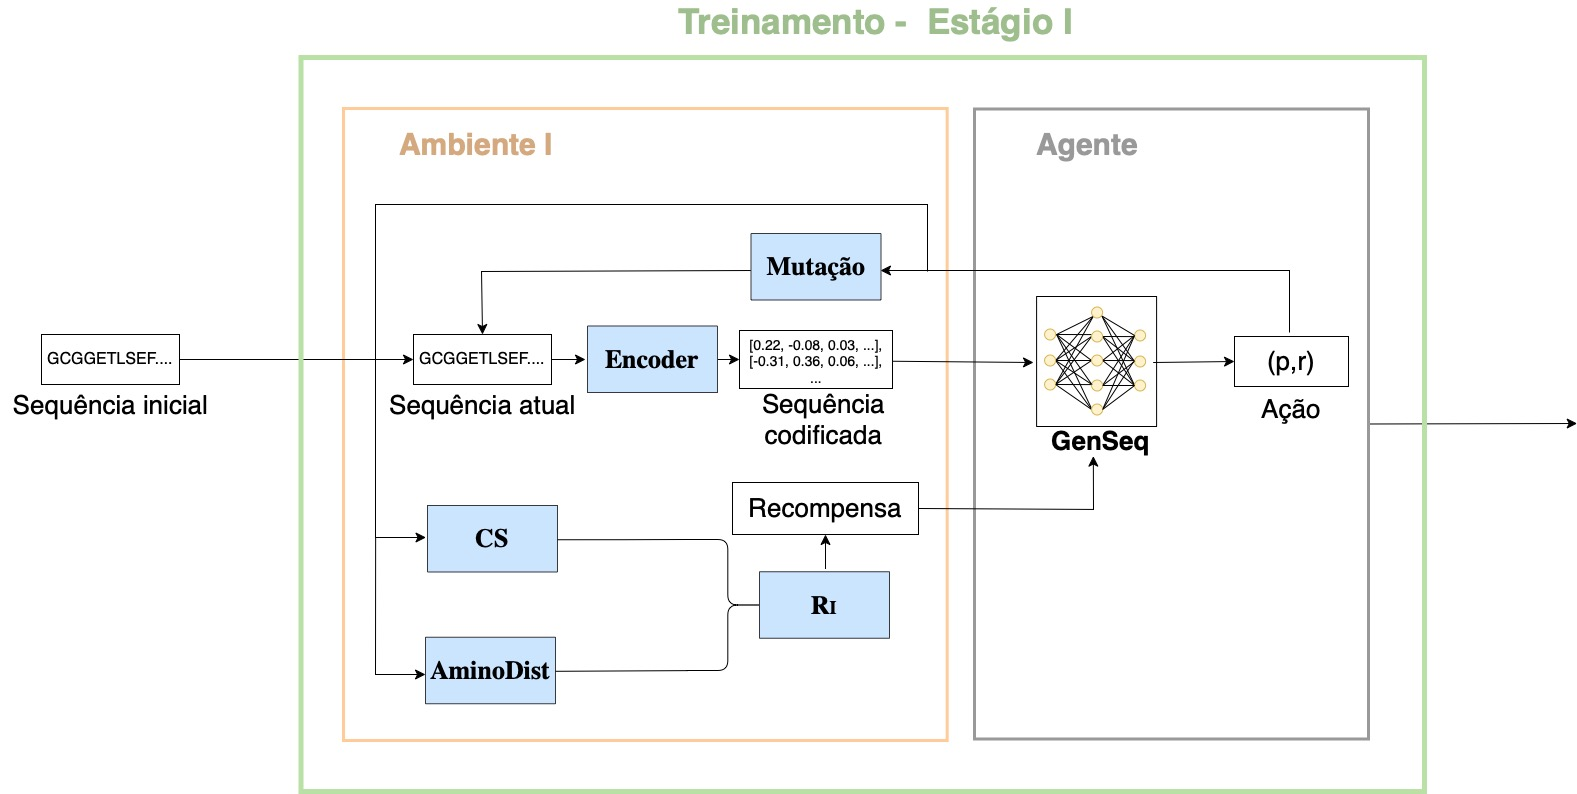
\includegraphics[width=.9\textwidth]{figuras/metodologia-Pre-Training.jpg}
  \caption{Primeiro estágio de treinamento}
\end{figure}


Neste estágio, o Agente foi treinado com um total de 2 milhões de iterações, podendo executar até 100 mutações por episódio.
\begin{table}[H]
  \centering
  \vspace{0.5cm}
  \begin{tabular}{r|lr}
  Parâmetro & Valor \\ 
  \hline                               % para uma linha horizontal
  Número máximo de mutações por episódio & 100 \\
  Número de iterações & 2.000.000 \\
  Tamanho do \textit{batch} & 200 \\
  $N_{rep}$ & 7 \\
  \end{tabular}
  \caption{Parâmetros preliminares}
  \end{table}

  Após finalizado o primeiro estágio, comparamos o desempenho do \textit{GenSeq} com o desempenho de uma política que define ações aleatoriamente, onde observamos
  que a mediana da distribuição de recompensas do \textit{GenSeq} é consideravelmente superior ao do Agente aleatório. 

  \begin{figure}[H]
    \centering
    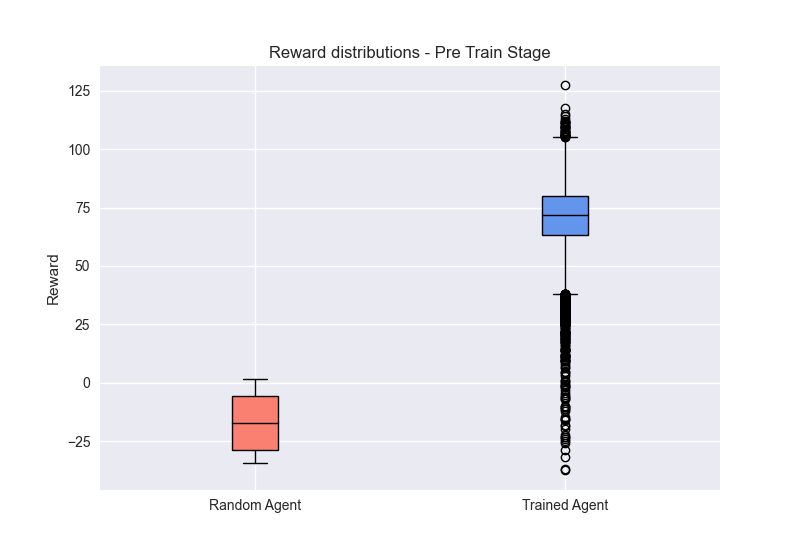
\includegraphics[width=.8\linewidth]{figuras/plot_box_pre_train_reward.jpg}  
    \caption{Comparação do Agente pré treinado com um Agente aleatório}
    \label{fig:box-pre-train}
  \end{figure}

Observa-se que o \textit{GenSeq} atingiu um platô de recompensas neste ambiente com cerca de 2500 episódios, como ilustrado em 
\ref{fig:rew_per_ep_pretrain}.

  \begin{figure}[H]
    \centering
    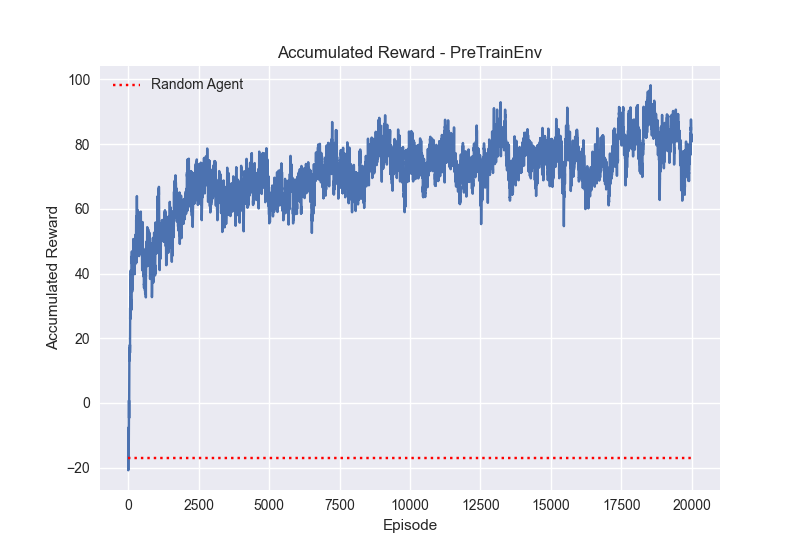
\includegraphics[width=.8\linewidth]{figuras/plot_pre_train_reward.jpg}    
    \caption{Média móvel das recompensas por episódio - treino}
    \label{fig:rew_per_ep_pretrain}
  \end{figure}


\subsection{Treinamento - Estágio II}
\label{subsection:stage2}
%Função do reward
%Numero de steps total e por episodio
%Vitoria ou derrota no episodio
O objetivo do segundo estágio de treinamento é fazer com que o agente pré treinado aprenda a escolher ações
que maximizem o \textit{TM-Score} entre a estrutura gerada e a alvo, 
i.e, minimizem o erro $1-TMScore$.
Para isto, definimos a função de recompensa como a soma de 3 termos: 

\begin{equation}
\label{eq:eqR2}
    R_{II} = -aEr_{i} + b(Er_{0} - Er_{i}) + c(Er_{i-1} - Er_{i})
\end{equation}

\noindent
Onde $Er_{i}$ e $Er_{i-1}$ são os erros da iteração i e i-1 respectivamente, e $a, b$ e $c$ são constantes. 
O primeiro termo, $-aEr_{i}$, é a penalização pelo erro atual.
O segundo determina uma penalização se o erro atual for maior que o inicial e uma recompensa caso contrário.
Análogamente, o terceiro termo penaliza se o erro atual for maior que o anterior e recompensa se for menor.
Como o objetivo principal é encontrar sequências com erro menores que o inicial, atribuímos um peso maior ao segundo termo,
i.e, $b>a$ e $b>c$.
Além disso, consideramos $c>a$ para valorizar reduções do erro ao longo do episódio.  
Introduzimos também o conceito de vitória e derrota a cada episódio. 
Consideramos vitória caso o erro final seja menor que o inicial e derrota caso contrário. 
De modo a valorizar a vitória e penalizar a derrota, 
ao final de cada episódio é adicionado uma recompensa adicional dada por $2500(Er_{0} - Er_{f})$, 
onde $Er_{f}$ é o erro final, i.e, da última iteração do episódio. 
Cada episódio é finalizado ao se atingir um número máximo de iterações, ou um limiar de erro. 
Foi definido um limite superior para o erro $Er_{max}$ de modo a evitar que o Agente atinja erros muito grandes em um mesmo episódio,
e um limite inferior $Er_{min}$ para valorizar episódios em que o Agente foi capaz de encontrar "atalhos", i.e,
conseguiu reduzir o erro considerávelmente em poucas iterações.

O pior cenário em termos de recompensa para o agente é o caso em que limiar de erro máximo $Er_{max}$ ocorre antes de atingir o número máximo 
de iterações. Nesse caso, a recompensa adicional é dada pela sequinte expressão:

\begin{equation}
  \label{eq:R2adicional}
      R_{II} \gets R_{II} + 2500(Er_{0} - Er_{i}) + R_{II}(M_{max} - step_{id})
\end{equation}

Ou seja, um termo adicional de penalização,
$R_{II}(M_{max} - step_{id})$, é incluído na recompensa final.
Esse termo representa uma estimativa pessimista da recompensa total caso o agente fosse autorizado 
a completar todas as $M_{max}$ iterações. 
A suposição subjacente é que, nas iterações restantes $M_{max} - step_{id}$, 
o agente manteria o desempenho atual, ou seja, continuaria acumulando a mesma recompensa $R_{II}$ 
associada a um erro superior ao limite máximo $Er_{max}$. 
Isso desestimula fortemente trajetórias em que o erro excede $Er_{max}$ precocemente.


A inicialização do segundo ambiente $EnvII$ é feita da mesma forma que $EnvI$, porém com a inclusão da definição de $Er_{i}$ e $Er_{i-1}$ que 
iniciam iguais ao erro inicial $Er_{0}$. O ambiente é dependente de parâmetros como $S_{ini}$, a estrutura do FIX 
($E_{FIX}$), o erro inicial ($E_r{0}$), os limiares de erro $Er_{max}$ e $Er_{min}$, o \textit{Encoder},
$M_{max}$, $N_{rep}$ e os coeficientes da função de recompensa $(a, b, c)$.

O método \textit{step} do $EnvII$, assim como no primeiro ambiente, recebe como entrada uma ação $(p, r)$
que é utilizada para realizar a mutação na sequência $S$. 
Posteriormente, a sequência é transformada
em uma representação codificada pelo $Encoder$, originando a $S_{enc}$.
É feita então a predição da estrutura tridimensional $E_S$ associada a sequência $S$ utilizando o modelo \textit{ESMFold}.
O erro da iteração anterior recebe o erro atual, que por sua vez, é atualizado com o resultado de $1-TMScore(E_{FIX}, E_{S})$.
Tendo $Er_{i}$ e $Er_{i-1}$, é calculado a recompensa $R_{II}$ seguindo a equação \ref{eq:eqR2}.
A atualização de $P_{val}$ e $R_{val}$ é realizada com a mesma lógica utilizada em $EnvII$.
Já o método \textit{reset} pouco difere do método implementado em $EnvI$. A única alteração consiste na atribuição do erro inicial 
para $Er_{i}$ e $Er_{i-1}$.


\begin{algorithm}[H]
  \caption{Ambiente de Aprendizado - Estágio II}
  \label{alg:EnvII}
  \begin{algorithmic}[1]
  \Require Classe $gym.ENV$, 
  \State         Condições iniciais $S_{ini}$ e $Er_{0}$
  \State         Estrutura do FIX $E_{FIX}$, 
  \State         Limiares de erro $Er_{min}$ e $Er_{max}$,
  \State         encoder $Encoder$,
  \State         número máximo de mutações por episódio $M_{max}$, 
  \State         número máximo de repetições do mesmo aminoácido por episódio $N_{rep}$,
  \State         coeficientes da função de recompensa $(a, b, c)$
  \Ensure Classe $EnvII$

  \State \textbf{class} $EnvII$ \textbf{herda} $gym.ENV$
  \State \quad $S \gets S_{ini}$
  \State \quad $Er_{i}, Er_{i-1} \gets Er_{0}$
  \State \quad $P_{val} \gets \textit{Todas as posições na sequência}$
  \State \quad $R_{val} \gets \textit{Todos os aminoácidos}$
  \State \quad $step_{id} \gets 0$

  \Function{reset()}{}
      \State $S \gets S_{ini}$
      \State $Er_{i}, Er_{i-1} \gets Er_{0}$
      \State $P_{val} \gets \textit{Todas as posições na sequência}$
      \State $R_{val} \gets \textit{Todos os aminoácidos}$
      \State $step_{id} \gets 0$
  \EndFunction

  \Function{step($(p,r)$)}{}
      \State $S \gets$ inserir $r$ na posição $p$ de $S$
      \State $S_{enc} \gets encoder(S)$
      \State $E_{S} \gets ESMFold(S)$
      \State $Er_{i-1} \gets Er_{i}$
      \State $Er_{i} \gets 1 - TMScore(E_{FIX}, E_{S})$
      \State $R_{II} \gets -aEr_{i} + b(Er_{0} - Er_{i}) + c(Er_{i-1} - Er_{i})$
      
      \If{$p \in P_{val}$}
          \State Remover $p$ de $P_{val}$
      \EndIf

      \If{$r$ já foi escolhido $N_{rep}$ vezes}
          \State Remover $r$ de $R_{val}$
      \EndIf

      \State $step_{id} \gets step_{id} + 1$
      \State $done \gets \textit{False}$

      \If{$step_{id} \geq M_{max}$ ou $Er_{i} \leq Er_{min}$ ou $Er_{i} \geq Er_{max}$}
          \State $done \gets \textit{True}$
          \If{$step_{id} = M_{max}$}
              \State $R_{II} \gets R_{II} + 2500(Er_{0} - Er_{i})$
          \EndIf
          \If{$Er_{i} \geq Er_{max}$}
              \State $R_{II} \gets R_{II} + 2500(Er_{0} - Er_{i}) + R_{II}(M_{max} - step_{id})$ 
          \EndIf
      \EndIf

      \State \Return $S_{enc}, R_{II}, done$
  \EndFunction

  \end{algorithmic}
\end{algorithm}

O \textit{loop} de treinamento segue a mesma lógica do primeiro estágio, alterando apenas o ambiente de aprendizado de 
$EnvI$ para $EnvII$ e suas respectivas dependências. 
Além disso, o treinamento se inicia com os pesos do \textit{GenSeq} pré treinados, obtidos através do primeiro estágio. 

\begin{algorithm}[H]
  \caption{Treinamento - Estágio II}
  \label{alg:train_stage2}
  \begin{algorithmic}[1]
  \Require Número total de iterações $N_{iter}$, 
  \State         número máximo de mutações por episódio $M_{max}$, 
  \State         Condições iniciais $S_{ini}$ e $Er_{0}$
  \State         encoder $Encoder$,
  \State         tamanho do batch $batch_size$,
  \State         coeficientes da função de recompensa $(a, b, c)$,
  \State         número máximo de repetições do mesmo aminoácido por episódio $N_{rep}$
  \State         Estrutura do FIX $E_{FIX}$, 
  \State         Limiares de erro $Er_{min}$ e $Er_{max}$,
  \State         Agente pré treinado \textit{GenSeq}
  \Ensure Agente treinado \textit{GenSeq}
  \State $env \gets EnvII(S_{ini}, Er_{0}, Encoder, (a, b, c), E_{FIX}, Er_{min},Er_{max}, M_{max}, N_{rep})$ 
  \State $S_{enc} \gets Encoder(S_{ini})$ 
  \State $R_{hist} \gets []$ 
  \For{$i = 1$ to $N_{iter}$}
      \State $(p,r) \gets GenSeq(S_{enc})$ 
      \State $(S_{enc}, R_{II}, done) \gets env.step(p, r)$ 
      \State Adiciona $R_{II}$ ao $R_{hist}$ 
      \If{done = True}
          \State $env.reset()$ 
      \EndIf
      \If{i mod batch\_size = 0}
          \State Atualizar pesos do GenSeq baseado em $R_{hist}$ utilizando PPO
          \State $R_{hist} \gets []$
      \EndIf
  \EndFor
  \State \Return $GenSeq$
  \end{algorithmic}
\end{algorithm}

A implementação do $EnvII$\footnote{Disponível em: \url{https://github.com/ArthurPimenta0306/Hallucination/blob/main/hpd/src/hpd/pipelines/RLenvs/nodes.py}}
bem como do segundo estágio de treinamento\footnote{Disponível em: \url{https://github.com/ArthurPimenta0306/Hallucination/blob/main/hpd/src/hpd/pipelines/Modeling/nodes.py}}
estão disponíveis. 
A figura a seguir ilustra uma visão geral da relação entre o segundo ambiente de aprendizagem e o 
agente durante o segundo estágio de treinamento.

\begin{figure}[H]
  \centering
  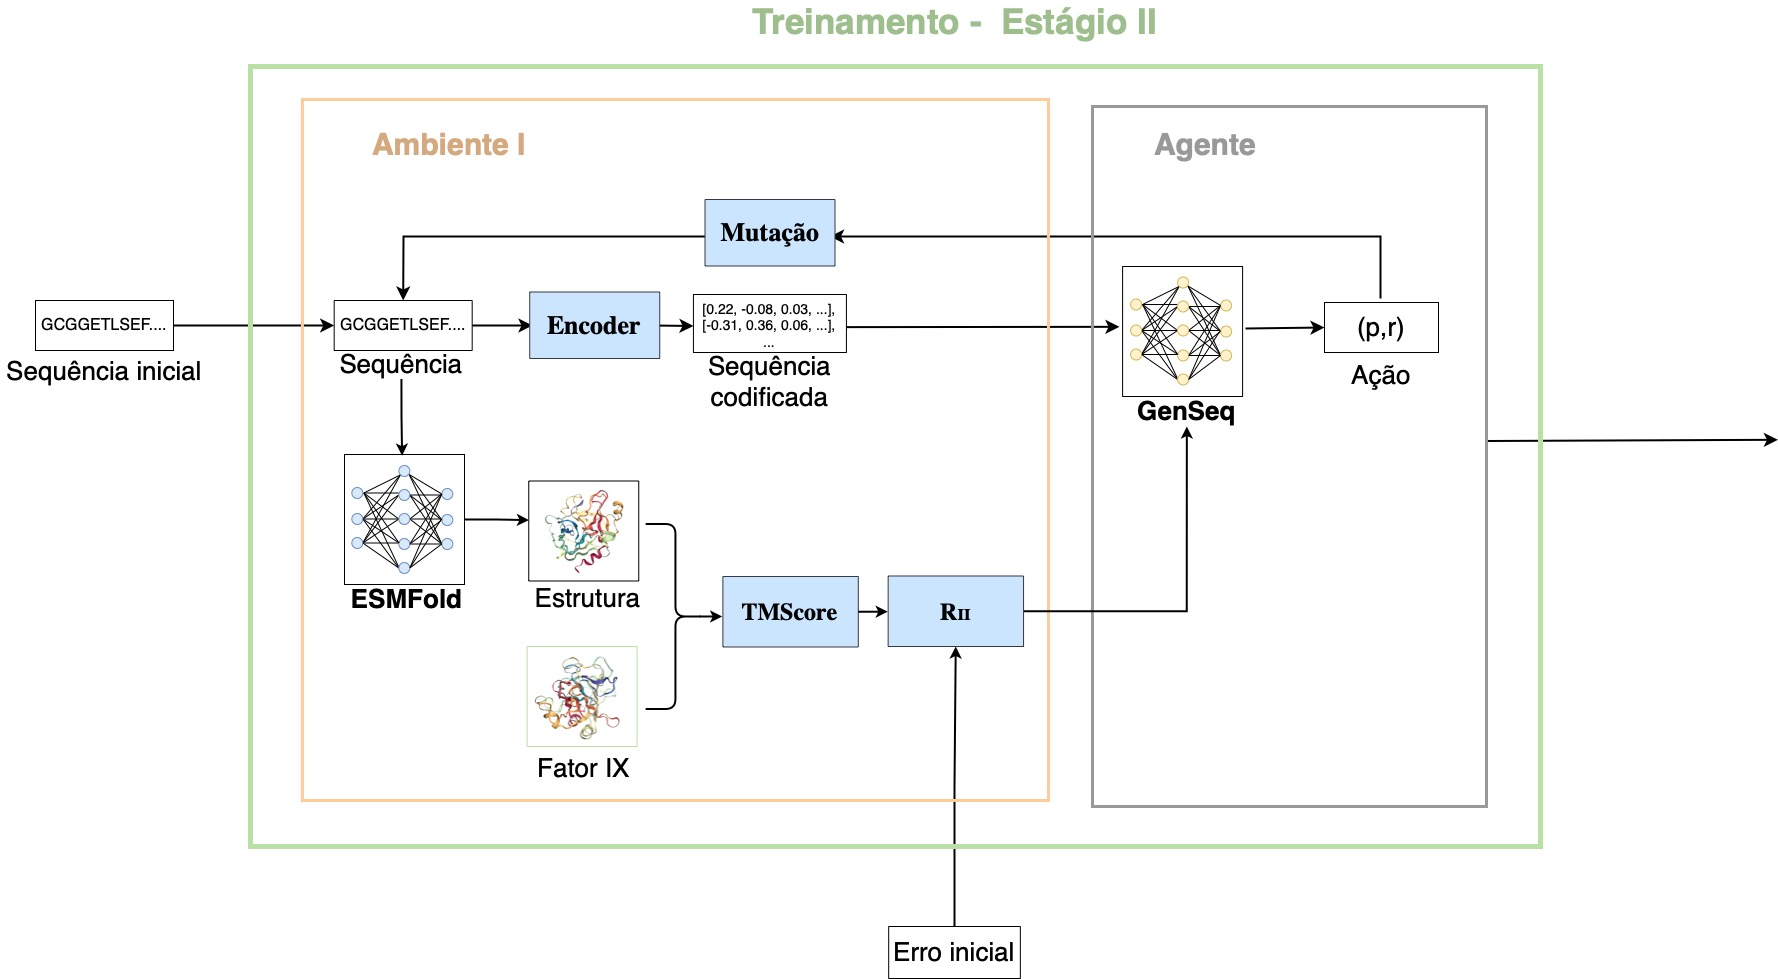
\includegraphics[width=.8\textwidth]{figuras/metodologia-Training.jpg}
  \caption{Segundo estágio - Treino}
\end{figure}

Neste estágio, o Agente foi treinado com um total de 60 mil de iterações, podendo executar até 45 mutações por episódio. 

\begin{table}[H]
  \centering
  \vspace{0.5cm}
  \begin{tabular}{r|lr}
  Parâmetro & Valor \\ 
  \hline                               % para uma linha horizontal
  Número máximo de mutações por episódio & 45 \\
  Erro mínimo no episódio & 0.05 \\
  Erro máximo no episódio & 0.083 \\
  Número de iterações & 60.000 \\
  a & 12 \\
  b & 200 \\
  c & 50 \\
  $N_{rep}$ & 7 \\
  \end{tabular}
  \caption{Parâmetros preliminares}
  \end{table}

  Assim como no pré treino, a distribuição das recompensas do Agente ao longo do treinamento é 
  bem superior às recompensas de um Agente aleatório.  
  \begin{figure}[H]
    \centering
    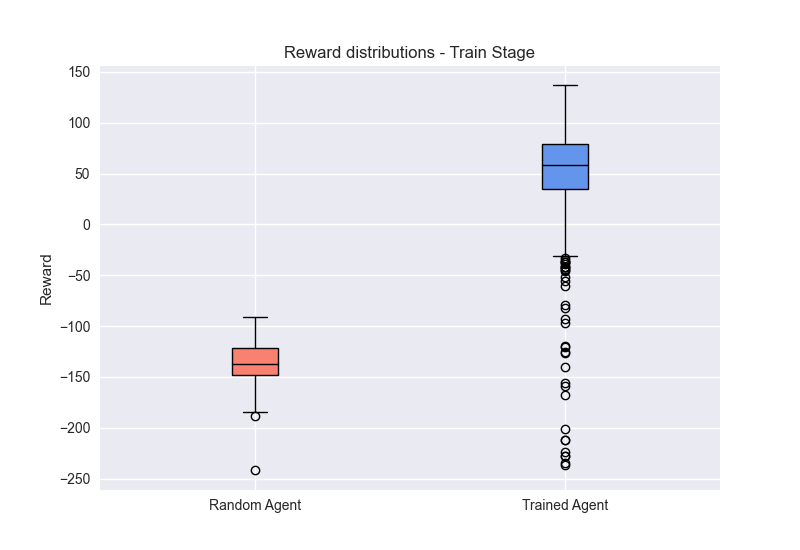
\includegraphics[width=.9\linewidth]{figuras/plot_box_train_reward.jpg}  
    \caption{Comparação do Agente treinado com um Agente aleatório}
    \label{fig:box-train}
  \end{figure}

  Repare que, devido ao pré treino, as recompensas médias do Agente são consideravelmente superiores
  à recompensa média do Agente aleatório desde os primeiros episódios. 
  \begin{figure}[H]
    \centering
    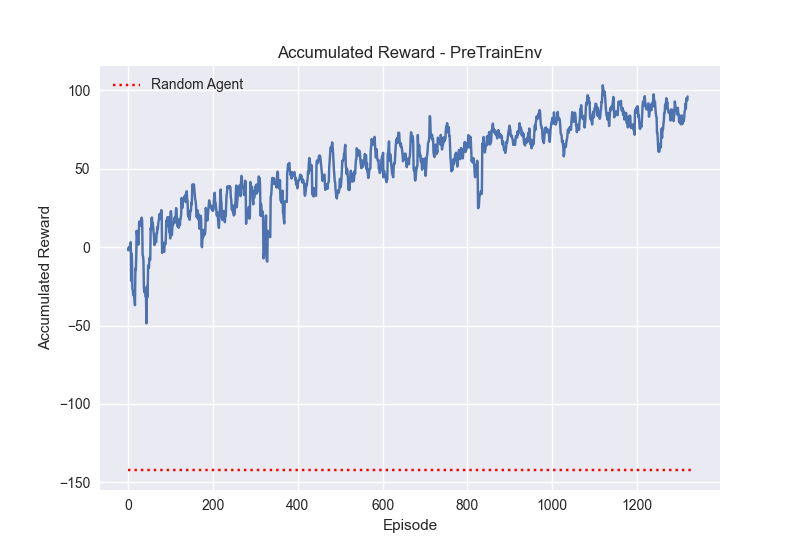
\includegraphics[width=.8\linewidth]{figuras/plot_train_reward.jpg}    
    \caption{Média móvel das recompensas por episódio - treino}
    \label{fig:rew_per_ep_train}
  \end{figure}
  

\section{Geração de sequências}
Por fim, o módulo de Geração de Sequências utiliza o agente treinado para gerar novas 
sequências que sejam capazes de mimetizar a estrutura alvo melhor do que a sequência inicial, em termos de \textit{TMScore}.  
Para isso, o ambiente $EnvII$ é inicializado com as mesmas condições utilizadas no segundo estágio de treinamento,
incluindo a sequência inicial $S_{ini}$, o erro inicial $Er_{0}$, o $Encoder$, os coeficientes $(a, b, c)$ 
e a estrutura alvo $E_{FIX}$.
Para maximizar a diversidade de sequências geradas,
as restrições impostas pelos limiares de erro $Er_{min}$ e $Er_{max}$ são removidas, 
sendo definidos como 0 e 1, respectivamente. 
Além disso, a geração de sequências é configurada para produzir um total de 235 novas variantes, 
fixando os parâmetros $N_{iter}$ e $M_{max}$ em 235.
O processo de geração consiste em iterativamente obter uma ação com o \textit{GenSeq} 
e com ela executar o método \textit{step} no $EnvII$.

\begin{algorithm}[H]
  \caption{Geração de sequências}
  \label{alg:gerseq}
  \begin{algorithmic}[1]
  \Require Número total de iterações $N_{iter}$, %235
  \State         número máximo de mutações por episódio $M_{max}$, %235
  \State         Condições iniciais $S_{ini}$ e $Er_{0}$
  \State         encoder $Encoder$,
  \State         coeficientes da função de recompensa $(a, b, c)$,
  \State         número máximo de repetições do mesmo aminoácido por episódio $N_{rep}$
  \State         Estrutura do FIX $E_{FIX}$, 
  \State         Limiares de erro $Er_{min}$ e $Er_{max}$, %0 e 1
  \State         Agente treinado \textit{GenSeq}
  \Ensure Novas sequências $Seqs$
  \State $env \gets EnvII(S_{ini}, Er_{0}, Encoder, (a, b, c), E_{FIX}, Er_{min},Er_{max}, M_{max}, N_{rep})$ 
  \State $S_{enc} \gets Encoder(S_{ini})$ 
  \State $Seqs \gets []$ 
  \For{$i = 1$ to $N_{iter}$}
      \State $(p,r) \gets GenSeq(S_{enc})$ 
      \State $(S_{enc}, R_{II}, done) \gets env.step(p, r)$ 
      \State Adiciona $env.S$ ao $Seqs$ 
  \EndFor
  \State \Return $Seqs$
  \end{algorithmic}
\end{algorithm}

A implementação da geração de sequências está disponível\footnote{Disponível em: \url{https://github.com/ArthurPimenta0306/Hallucination/blob/main/hpd/src/hpd/pipelines/Evaluation/nodes.py}}.
A figura a seguir representa um esquemático do \textit{loop} de geração de sequências descrito.

\begin{figure}[H]
  \centering
  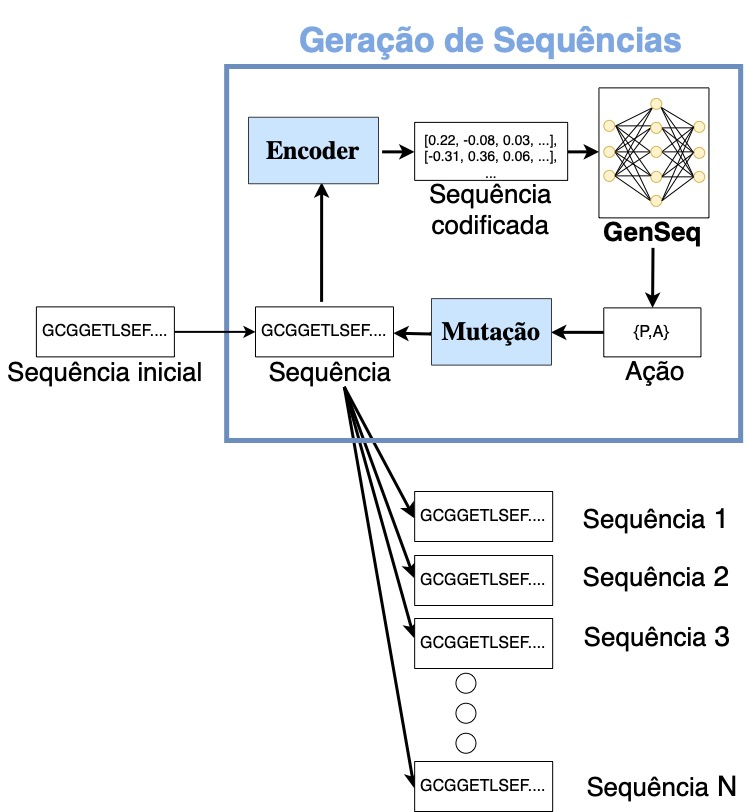
\includegraphics[width=.8\textwidth]{figuras/metodologia-Generating.jpg}
  \caption{Gerando sequência otimizada}
  \label{fig:geradorseq}
\end{figure}


\section{Métodos de avaliação}
{\color{red} Em andamento}
{\color{red} TMScore, Docking e imuno}

